\documentclass[conference]{IEEEtran}
\IEEEoverridecommandlockouts
\usepackage{cite}
\usepackage{amsmath,amssymb,amsfonts}
\usepackage{algorithm}
\usepackage{algpseudocode}
\usepackage{graphicx}
\usepackage{textcomp}
\usepackage{xcolor}
\usepackage{booktabs}
\usepackage{multirow}
\usepackage{array}
\usepackage{tabularx}
\usepackage{tikz}
\usetikzlibrary{positioning,arrows.meta}
\usepackage{url}
\def\BibTeX{{\rm B\kern-.05em{\sc i\kern-.025em b}\kern-.08em
    T\kern-.1667em\lower.7ex\hbox{E}\kern-.125emX}}

% generated by code/experiments/make_tables.py
\newcommand{\BestOtherEvent}{SVM}
\newcommand{\BestOtherEventFone}{0.620}
\newcommand{\EventPurity}{0.83}
\newcommand{\KUeventAcc}{0.587}
\newcommand{\KUeventAuc}{0.633}
\newcommand{\KUeventFone}{0.543}
\newcommand{\KUrandomAcc}{0.692}
\newcommand{\KUrandomAuc}{0.755}
\newcommand{\KUrandomFone}{0.686}
\newcommand{\KUseqeventAcc}{0.598}
\newcommand{\KUseqeventAuc}{0.653}
\newcommand{\KUseqeventFone}{0.565}
\newcommand{\KUseqrandomAcc}{0.718}
\newcommand{\KUseqrandomAuc}{0.781}
\newcommand{\KUseqrandomFone}{0.712}
\newcommand{\LatencyRatio}{10.6}
\newcommand{\LookupeventAcc}{0.524}
\newcommand{\LookupeventAuc}{0.500}
\newcommand{\LookupeventFone}{0.344}
\newcommand{\LookuprandomAcc}{0.769}
\newcommand{\LookuprandomAuc}{0.837}
\newcommand{\LookuprandomFone}{0.768}
\newcommand{\VFLeventAcc}{0.600}
\newcommand{\VFLeventAuc}{0.649}
\newcommand{\VFLeventFone}{0.593}
\newcommand{\VFLrandomAcc}{0.792}
\newcommand{\VFLrandomAuc}{0.878}
\newcommand{\VFLrandomFone}{0.791}
\newcommand{\VFeventAcc}{0.638}
\newcommand{\VFeventAuc}{0.687}
\newcommand{\VFeventFone}{0.628}
\newcommand{\VFrandomAcc}{0.702}
\newcommand{\VFrandomAuc}{0.775}
\newcommand{\VFrandomFone}{0.699}
\providecommand{\LookupRandomFone}{0.768}
\providecommand{\LookupEventFone}{0.344}
   % macros with every reported result (generated from results/tables/*.csv)

\begin{document}

\title{VeriFlux: Lightweight, Event-Aware and Explainable Fake News Detection from Social Signals on the KeepUp Dataset}

\author{\IEEEauthorblockN{M. Shah Nawaz}
\IEEEauthorblockA{\textit{Dept. of Software Engineering} \\
\textit{FAST-NUCES, Chiniot--Faisalabad Campus}\\
Chiniot, Pakistan \\
f233077@cfd.nu.edu.pk}
\and
\IEEEauthorblockN{M. Hamza Ismail}
\IEEEauthorblockA{\textit{Dept. of Software Engineering} \\
\textit{FAST-NUCES, Chiniot--Faisalabad Campus}\\
Chiniot, Pakistan \\
f233109@cfd.nu.edu.pk}
}

\maketitle

% ===========================================================================
\begin{abstract}
Fake news on social media is now detected by systems that combine the post text with external evidence,
the stance of comments, the profile of the author and engagement counts. KeepUp is a recent framework of this
kind for multilingual and Urdu content, but it is computationally heavy, its decisions are not explained, and
it was evaluated on a random split of posts. Because many posts in KeepUp describe the same event, a random
split places near-duplicate stories in both training and test data. We show that a rule which only returns the
majority label of a post's event reaches a macro-F1 of \LookupRandomFone{} under a random split but only
\LookupEventFone{} when whole events are held out. We therefore re-implement KeepUp and thirteen baselines
under one protocol in which test events are never seen during training, and propose VeriFlux. VeriFlux pairs a
frozen multilingual text embedding and 38 named evidence, stance, user, engagement and title features with an
event-context contrast that compares each post with the other posts about the same claim, and classifies the
result with a kernel support vector machine. A transformer-free variant, VeriFlux-Lite, uses gradient boosting
and is explained with TreeSHAP. On unseen events VeriFlux obtains the best macro-F1 (\VFeventFone{}) and AUC
(\VFeventAuc{}) of all eighteen models, significantly above KeepUp (\KUeventFone{}), while running
\LatencyRatio{} times faster on a laptop CPU. VeriFlux-Lite gives the best random-split macro-F1
(\VFLrandomFone{}). The results show that honest, low-cost evaluation is essential before such detectors are
deployed.
\end{abstract}

\begin{IEEEkeywords}
fake news detection, social context, event-held-out evaluation, data leakage, explainable AI, Urdu
\end{IEEEkeywords}

% ===========================================================================
\section{Introduction}
Social media platforms have become a primary source of news for a large share of internet users, and in
countries such as Pakistan a single misleading post about health, politics or religion can be reshared
thousands of times within hours. Fake news on these platforms is rarely a plain article: it is a short,
often code-mixed post that sits inside a network of comments, reactions and authors with different
credibility. The base paper of this study, KeepUp \cite{wasim2026keepup}, released a dataset that captures
this setting for English, Urdu and Roman Urdu content and proposed a unified framework to exploit it.

Detection research has moved in the same direction, from text-only classifiers towards systems that combine
external evidence, comment stance, user profiles and propagation patterns
\cite{wasim2026keepup,almutair2025msdsi,nivedita2026hgcm}. KeepUp follows this trend: it retrieves evidence
with a dense multilingual retriever, scores entailment with a large language model, classifies the stance of
every comment with a fusion network and combines all signals in a CNN and BiGRU model, reporting an accuracy
and F1 of 0.78.

Two properties of this result motivate our work. First, the score was obtained with a single random split
of posts. In KeepUp, posts are grouped around 172 events (a median of four posts per event), and the labels
inside an event are highly uniform (label purity \EventPurity). A random split therefore places posts about
the same claim in both training and test data. To measure the effect, we evaluated a trivial rule that
predicts the majority training label of a post's event: it reaches a macro-F1 of \LookupRandomFone{} on random
splits, close to KeepUp's reported score, but only \LookupEventFone{} when events are held out. Second, the
framework requires several transformer models per post, including a stance network applied to every comment,
yet its computational cost is not reported and its predictions are not explained.

Our literature review of fifteen 2025--2026 journal articles found the same pattern across the field. Models
that use rich social context are heavy and rarely explained; runtime is reported only for text-only models;
almost all studies use random splits, and only one tests on unseen events; and Urdu studies do not use social
signals at all. The objectives of this work are therefore to:
\begin{itemize}
\item reproduce KeepUp and the baselines it compares against under a single, leakage-free protocol;
\item quantify how much of the reported accuracy is explained by event memorisation;
\item design a lightweight and explainable detector that generalises to events not seen in training;
\item measure the cost, explanation quality and language-specific behaviour of every model.
\end{itemize}

The proposed solution, VeriFlux (Fig.~\ref{fig:framework}), keeps KeepUp's four signal families but replaces
its expensive components with compact alternatives: BM25 retrieval with a small multilingual NLI model, a
light cross-fitted stance classifier and a single frozen document embedding. Its main idea is an
\emph{event-context contrast}: every post is compared with the other, unlabelled posts about the same claim,
which removes claim-level offsets that a model would otherwise memorise. The contributions are as follows.
\begin{itemize}
\item An independent reproduction of KeepUp (two variants) and thirteen baselines on identical folds, with
every deviation documented. Our best KeepUp variant reaches a random-split macro-F1 of \KUseqrandomFone{} against
the reported 0.78.
\item A leakage analysis showing that every model loses between 0.066 and 0.198 macro-F1 when events are held
out, and that an event lookup rule nearly matches the published KeepUp score on random splits.
\item VeriFlux, which achieves the best event-held-out macro-F1 (\VFeventFone{}) and AUC (\VFeventAuc{}) of
all models, a significant gain of 0.085 macro-F1 over KeepUp (Wilcoxon $p=0.003$), and the transformer-free
VeriFlux-Lite, which is the best model under random splits (\VFLrandomFone{}).
\item A cost, explanation, comment-budget and language analysis: VeriFlux is \LatencyRatio{} times and
VeriFlux-Lite 29.5 times faster than KeepUp per post on a laptop CPU, and the TreeSHAP explanations are
faithful (removing the single top feature changes the prediction seven times more than removing a random one).
\end{itemize}

The rest of the paper is organised as follows. Section~\ref{sec:lit} reviews related work,
Section~\ref{sec:method} describes VeriFlux, Section~\ref{sec:setup} gives the experimental setup,
Section~\ref{sec:results} reports the results, and Sections~\ref{sec:discussion}--\ref{sec:conclusion}
discuss the findings, limitations and conclusions.

% ===========================================================================
\section{Literature Review and Related Work}
\label{sec:lit}
We reviewed fifteen journal articles published in 2025 and 2026 together with the base paper. They are
grouped into five themes below and compared in Table~\ref{tab:lit}.

\subsection{Unified multi-signal detection (base paper)}
KeepUp \cite{wasim2026keepup} addresses fake news detection on Facebook, Instagram, X and YouTube posts
written in English, Urdu, Roman Urdu and three other languages. Its pipeline retrieves evidence for each
claim with BGE-M3 and a re-ranker, scores claim--evidence entailment with NorGLM, classifies the stance of each
comment with an XLM-R based fusion network (XStanceFusion), and combines the resulting counts with user,
engagement and title features in a CNN and BiGRU network. The released dataset contains 1,024 annotated posts,
about 70 thousand comments and nearly 12 thousand evidence documents. The authors report 0.78 accuracy and F1
and 0.84 AUC, ahead of classical, recurrent and transformer baselines. The evaluation, however, uses one random
post split, the computational cost of the five-model pipeline is not reported, and no per-decision explanation
is given.

\subsection{Efficiency and lightweight detection}
EPRVFL \cite{gurjwar2025eprvfl} feeds BERT embeddings into a shallow random-vector functional-link network and
reaches millisecond-level inference on PolitiFact, LIAR2 and BuzzFeed, showing that a light classifier on top of
a frozen encoder can be competitive. Elbaghazaoui et al. \cite{elbaghazaoui2025comparative} compare gradient
boosting, XGBoost and support vector classifiers on ISOT and report near-perfect accuracy together with training
time, and Mouratidis et al. \cite{mouratidis2025misinformation} benchmark TF-IDF and BERT pipelines with SHAP and
LIME on four article datasets. All three studies measure cost or explanation, but only on article text, which
is far easier than short social posts and contains no social context.

\subsection{User profiling and social context}
MSDSI-FND \cite{almutair2025msdsi} combines linguistic, user and cascade features of influential COVID-19 posts
and reports an AUC of 0.994, although on only 68 root posts. HGCM-Net \cite{nivedita2026hgcm} builds a
user--content graph with graph attention and contrastive learning and reaches 97.1\% accuracy on FakeNewsNet;
the authors note that sparse user graphs cause most errors. SiMiD \cite{ozcelik2025simid} adds community
information from the follower graph to a contrastive transformer, and Phan et al. \cite{phan2025context} combine
BERT content features with a dependency-graph network. These works confirm that social context helps, but each
relies on large graphs or several deep encoders, and none reports runtime.

\subsection{Evidence, stance and context}
HCFND \cite{kumar2025hcfnd} retrieves context through hashtags and named entities and improves over earlier
detectors, but it depends on posts that carry hashtags. Sun et al. \cite{sun2025evolving} model how the stance of
replies evolves over time inside a multimodal graph and show that stance dynamics are informative for rumour
detection, at the cost of a heavy multimodal architecture. Together with KeepUp, these studies motivate the
evidence and stance families in our model, while pointing to the need for cheaper extractors.

\subsection{Early detection and cross-event generalisation}
LDPG \cite{ji2026ldpg} builds local propagation graphs over time windows and remains accurate when only early
reactions are available, but it requires timestamped propagation data and images. EvolveDetector
\cite{ding2025evolvedetector} is the only reviewed study that explicitly tests on emerging events: it
accumulates event knowledge through continual learning and outperforms static detectors on new events from X
and Weibo, although it uses content alone.

\subsection{Explainable, multilingual and Urdu detection}
HEMT-Fake \cite{jadhav2025hemtfake} fuses four encoders for multilingual and multimodal news and validates its
explanations with a human study, but it does not cover Urdu. For Urdu, Harris et al. stack three transformers
\cite{harris2025urduensemble} and fine-tune a 7-billion-parameter LLaMA-2 model with LoRA on a new 78-thousand
article corpus \cite{harris2025hookbait}, and Farooq et al. \cite{farooq2025urdu} compare classical, deep and
large language models on two Urdu benchmarks. All three Urdu studies classify article text only and ignore the
social signals that KeepUp provides.

\subsection{Comparative analysis and research gap}
Table~\ref{tab:lit} summarises the reviewed work. The studies that exploit social context (KeepUp, MSDSI-FND,
HGCM-Net, SiMiD, HCFND, LDPG) are also the heaviest, and none of them reports computational cost or a faithful
explanation, while the studies that do report cost (EPRVFL and the comparative work) use only article text.
Most evaluations rely on random splits, so a model can succeed by recognising the story rather than judging the
post; only EvolveDetector measures performance on unseen events. Finally, Urdu detection research has not yet
used comments, users or engagement. The central gap is therefore the lack of a social-context fake news
detector for multilingual and Urdu posts that is evaluated on unseen events, runs at low cost on a CPU and
explains its decisions.

% Condensed from the authors' own literature review (Tables I-III). Re-check every cell against the papers.
\begin{table*}[t]
\centering
\caption{Comparative analysis of the reviewed 2025--2026 journal articles}
\label{tab:lit}
\scriptsize
\setlength{\tabcolsep}{3pt}
\begin{tabularx}{\textwidth}{>{\raggedright\arraybackslash}p{2.1cm} >{\raggedright\arraybackslash}X >{\raggedright\arraybackslash}p{2.6cm} >{\raggedright\arraybackslash}p{2.3cm} >{\raggedright\arraybackslash}p{2.6cm} >{\raggedright\arraybackslash}X c c c}
\toprule
Study & Method & Dataset & Evaluation & Key finding & Main limitation & Ctx & Cost & Ev.\\
\midrule
KeepUp \cite{wasim2026keepup} & BGE retrieval, NLI, XStanceFusion, CNN+BiGRU fusion & KeepUp (1,024 posts, 6 lang.) & Acc, P, R, F1, AUC & Acc/F1 0.78 & Random split; heavy; no cost or attribution & \checkmark & -- & -- \\
EPRVFL \cite{gurjwar2025eprvfl} & BERT + shallow RVFL & PolitiFact, LIAR2, BuzzFeed & Acc, F1, time & ms-level inference & Text only & -- & \checkmark & -- \\
Elbaghazaoui \cite{elbaghazaoui2025comparative} & GB, XGBoost, SVC & ISOT & Acc, time & 99.6\% acc. & Saturated article benchmark & -- & \checkmark & -- \\
Mouratidis \cite{mouratidis2025misinformation} & TF-IDF/BERT + ML/DL, SHAP, LIME & 4 article sets & F1, MCC, AUC & BERT F1 up to 0.99 & Article text; random splits & -- & -- & -- \\
HEMT-Fake \cite{jadhav2025hemtfake} & XLM-R, CNN-BiLSTM, ResNet, GraphSAGE & 74k articles, 5 lang. & Macro-F1, human study & +5\% macro-F1 & Four encoders; no Urdu & $\circ$ & -- & -- \\
MSDSI-FND \cite{almutair2025msdsi} & LIWC, user and cascade features + ML & 68 COVID-19 roots & Acc, F1, AUC & AUC 0.994 & Very small; one topic & \checkmark & -- & $\circ$ \\
HGCM-Net \cite{nivedita2026hgcm} & User--content graph, GAT, contrastive & FakeNewsNet & Acc, F1, MCC & Acc 97.1\% & Sparse-graph errors; heavy & \checkmark & -- & -- \\
SiMiD \cite{ozcelik2025simid} & Contrastive transformer + community & 3 X datasets & Weighted F1 & F1 $>$90\% & Needs follower graph & \checkmark & -- & -- \\
Phan et al. \cite{phan2025context} & BERT + dependency GCN & PolitiFact, GossipCop & Acc, F1 & +3 pp over SOTA & Two deep encoders & \checkmark & -- & -- \\
HCFND \cite{kumar2025hcfnd} & Hashtag/entity context retrieval & Social benchmarks & Classification & Beats SOTA & Needs hashtags & \checkmark & -- & -- \\
Sun et al. \cite{sun2025evolving} & Dynamic stance interaction, GNN & Rumour benchmarks & Classification & Stance evolution helps & Multimodal cost & \checkmark & -- & -- \\
LDPG \cite{ji2026ldpg} & Windowed propagation graphs & PHEME, PolitiFact, GossipCop & Early detection & Robust early & Images + graphs & \checkmark & -- & -- \\
EvolveDetector \cite{ding2025evolvedetector} & Continual learning, event memory & X, Weibo & Cross-event & Better on new events & Content only & -- & -- & \checkmark \\
Harris et al. \cite{harris2025urduensemble} & ELECTRA+mBERT+XLM-R stacking & UrduFake@FIRE & Acc, F1 & Ensemble best & 3 transformers & -- & -- & -- \\
Hook \& Bait \cite{harris2025hookbait} & LoRA LLaMA-2 7B & 78k Urdu + ISOT & Classification & Strong multilingual & 7B model cost & -- & -- & $\circ$ \\
Farooq et al. \cite{farooq2025urdu} & ML, DL, BERT, GPT-2 & Bend the Truth, Ax-to-Grind & Acc, F1 & Transformers best & No social context & -- & -- & -- \\
\midrule
\textbf{VeriFlux (ours)} & XLM-R embedding + 38 named features + event contrast + SVM; Lite: LightGBM + TreeSHAP & KeepUp & Event-held-out, cost, SHAP & see Sec.~\ref{sec:results} & -- & \checkmark & \checkmark & \checkmark \\
\bottomrule
\multicolumn{9}{l}{Ctx = social context used; Cost = runtime reported; Ev. = unseen-event evaluation. \checkmark\ yes, $\circ$ partial, -- no.}
\end{tabularx}
\end{table*}


% ===========================================================================
\section{Proposed Methodology}
\label{sec:method}
\subsection{Overview}
Fig.~\ref{fig:framework} shows the complete pipeline. The posts are first divided into folds by event, so that
every subsequent component is trained only on training events. For each claim, BM25 retrieves evidence that a
small multilingual NLI model compares with the claim and with the post title. A cross-fitted TF-IDF classifier
labels the stance of each comment, and the resulting proportions are combined with user, engagement and title
statistics into 38 named features. In parallel, a frozen XLM-R encoder produces one document embedding per
post. Both representations are paired with their event-context contrast and classified by an RBF support vector
machine (VeriFlux). The transformer-free VeriFlux-Lite replaces the embedding with an out-of-fold TF-IDF text
prior and uses LightGBM, whose predictions are explained exactly with TreeSHAP.

\begin{figure*}[t]
\centering
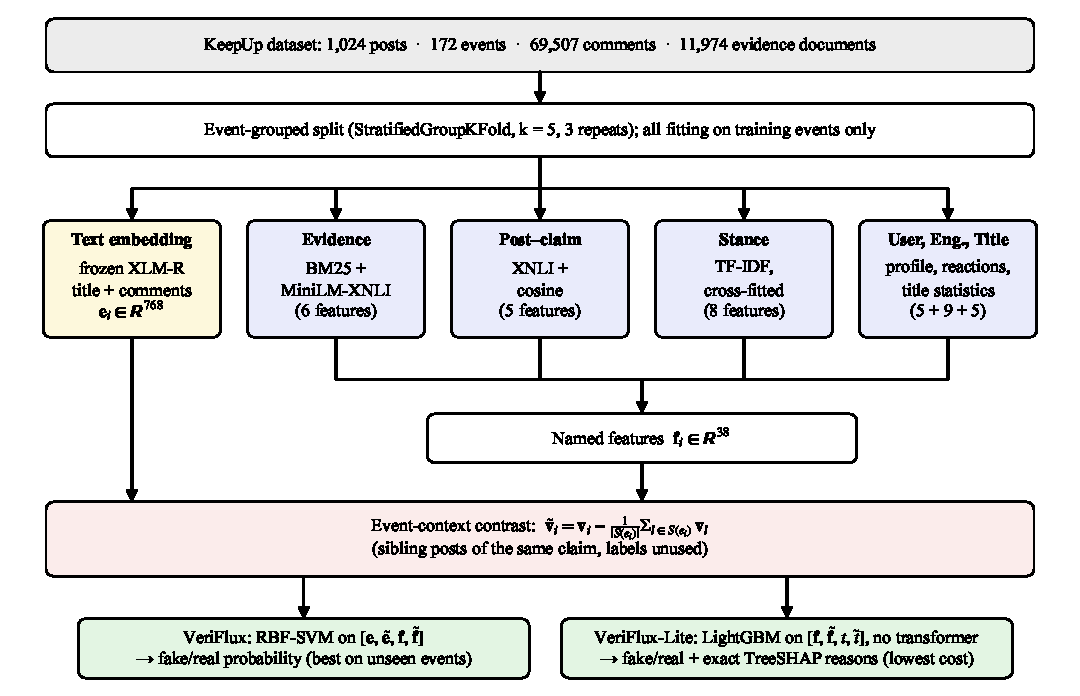
\includegraphics[width=0.95\textwidth]{figures/framework.pdf}
\caption{VeriFlux framework. Data are split by event before any model is fitted. A frozen text embedding and 38 named
features are paired with their event-context contrast and classified by an RBF-SVM (VeriFlux); the transformer-free
VeriFlux-Lite uses LightGBM on the named features and is explained with TreeSHAP.}
\label{fig:framework}
\end{figure*}

\subsection{Dataset and preparation}
We use the public KeepUp dataset (Table~\ref{tab:data}). It contains 1,024 labelled posts (537 fake and 487 real,
with label 1 denoting fake) about 172 events, 188 claims with 11,974 evidence documents, and 69,507 comments
annotated as agree, disagree, query or comment. Titles and comments were cleaned by removing URLs, user mentions
and hashtag symbols; code-mixed text was kept as written and not translated. Count variables such as likes,
followers and views were transformed with $\log(1+x)$. A language tag was assigned to each title by script:
Arabic script was tagged as Urdu, and Latin script was tagged as Roman Urdu when at least 10\% of its tokens
appear in a Roman-Urdu lexicon, otherwise as English. Several attributes are often missing (views for 48\% of
posts, shares for 52\% and the account joining date for 72\%); they were kept as missing values for the tree
models and median-imputed for the others.

\begin{table}[t]
\centering
\caption{KeepUp dataset as used in this study}
\label{tab:data}
\footnotesize
\begin{tabular}{lr}
\toprule
Property & Value\\
\midrule
Events with posts / claims & 172 / 188\\
Evidence documents & 11,974\\
Posts (fake / real) & 1,024 (537 / 487)\\
Posts per event (median / max) & 4 / 64\\
Label purity within events & 0.832\\
Comments (A / D / Q / C) & 69,507 (22,712 / 9,029 / 5,859 / 31,907)\\
Title script: Latin / Urdu & 691 / 332\\
Platforms (FB / IG / X / YT) & 417 / 254 / 220 / 124\\
\bottomrule
\end{tabular}
\end{table}


\subsection{Problem formulation}
We now fix the notation used in the rest of the section.
Let $\mathcal{D}=\{(p_i, e_i, y_i)\}_{i=1}^{N}$ be posts $p_i$ about event $e_i$ with label
$y_i\in\{0,1\}$ ($1=$ fake). Each event has a claim $c_{e}$, and each post has a comment set $C_i$.
A detector learns $f:\mathbf{x}_i\mapsto \hat{y}_i\in[0,1]$. Under the event-held-out protocol the
training and test sets satisfy
\begin{equation}
\{e_i : i\in\mathcal{T}_{\text{train}}\}\cap\{e_j : j\in\mathcal{T}_{\text{test}}\}=\varnothing .
\label{eq:eventsplit}
\end{equation}

\subsection{Feature families}
The named features follow the four signal families of KeepUp, but each family is computed with a component
that costs a fraction of the original.

\textbf{Evidence (6).} Evidence tells the model whether the claim behind a post is supported by trusted
sources. BM25 \cite{robertson2009bm25} retrieves the top-3 documents $d^{(1..3)}$ for claim $c$;
a 6-layer multilingual MiniLM NLI model \cite{wang2020minilm,conneau2018xnli} gives
$\mathbf{q}(d,c)=[P_E,P_N,P_C]$ with the evidence as premise. Features: $\mathbf{q}(d^{(1)},c)$,
$\max_k P_E(d^{(k)},c)$, $\max_k P_C(d^{(k)},c)$ and the BM25 score.

\textbf{Post--claim agreement (5).} A post may repeat a claim or argue against it, so the claim verdict alone
does not decide the label. With the claim as premise and the post title $t_i$ as hypothesis we compute
$\mathbf{r}_i=[P_E,P_N,P_C](c, t_i)$, the multilingual sentence-embedding cosine
$\cos(\phi(c),\phi(t_i))$ \cite{reimers2020multilingual}, and a veracity-consistency term motivated by
KeepUp's annotation guideline (a post is fake when it agrees with a false claim):
\begin{equation}
\kappa_i=\big(P_E(d^{(1)},c)-P_C(d^{(1)},c)\big)\cdot\big(P_E(c,t_i)-P_C(c,t_i)\big).
\label{eq:consistency}
\end{equation}

\textbf{Stance (8).} Readers often challenge false posts in the comments, as shown by the stance-based work in
Section~\ref{sec:lit}. A char/word TF-IDF logistic-regression stance classifier $g$ is cross-fitted over
events so that no comment is labelled by a model trained on its own event. For post $i$ and stance
$k\in\{A,D,Q,C\}$,
\begin{equation}
s_{ik}=\frac{|\{c\in C_i:\arg\max g(c)=k\}|}{\max(1,|C_i|)},
\label{eq:stance}
\end{equation}
plus $\log(1+|C_i|)$, a no-comment flag, the share of comments containing a 30-term debunk lexicon
(English, Roman Urdu, Urdu) and the doubt index $s_{iD}+s_{iQ}-s_{iA}$.

\textbf{User (5), engagement (9) and title (5).} Author credibility and audience reaction are the social
signals used by user-profiling studies \cite{almutair2025msdsi,nivedita2026hgcm}. We use log followers,
followings, account age and post count and the verification flag; log likes, comments, shares and views,
platform and media type; and title length, character count, Urdu script, URL and exclamation counts.

\subsection{Event-context contrast}
Posts about the same claim reach the platform together, and at inference time the other posts about a claim
are usually visible even when their labels are not. Raw features contain large claim-level offsets (for
example, all posts about one claim share the same evidence scores), and a classifier can memorise these offsets
instead of learning what separates a fake post from a real one. We therefore compare each post with its
unlabelled siblings. For any post-level vector $\mathbf{v}_i$ (text embedding or named features) the contrast
vector is
\begin{equation}
\tilde{\mathbf{v}}_{i}=\mathbf{v}_{i}-\frac{1}{|S(e_i)|}\sum_{l\in S(e_i)}\mathbf{v}_{l},
\label{eq:contrast}
\end{equation}
where $S(e_i)$ is the set of posts about event $e_i$ (training or test; labels unused). Because no label is
involved, the contrast does not leak test information, and Section~\ref{sec:results} shows that it is exactly
the claim-level memorisation that it removes which inflates random-split scores.

\subsection{VeriFlux classifier}
The dense text view is the mean-pooled embedding of the title and comments produced by a frozen XLM-R base
encoder \cite{conneau2020xlmr}. It is computed once per post, without fine-tuning, without a stance network over
every comment and without dense retrieval. The original vectors and their contrasts are concatenated and
standardised with training statistics:
\begin{equation}
\mathbf{z}_i=\big[\mathbf{e}_i,\ \tilde{\mathbf{e}}_i,\ \mathbf{f}_i,\ \tilde{\mathbf{f}}_i\big],\qquad
\hat{y}_i=\sigma\Big(a\sum_{j}\alpha_j y_j K(\mathbf{z}_j,\mathbf{z}_i)+b\Big),
\label{eq:z}
\end{equation}
with $K(\mathbf{z},\mathbf{z}')=\exp(-\gamma\lVert\mathbf{z}-\mathbf{z}'\rVert^2)$ and Platt-scaled
probabilities ($a,b$). This gives a 1,612-dimensional input ($2\times768+2\times38$). We chose a kernel
classifier because the training folds contain only about 800 posts: a maximum-margin model with an RBF kernel
is stable on small, high-dimensional data and has only two hyper-parameters, whereas deep fusion networks
overfit quickly at this scale.

\subsection{VeriFlux-Lite: transformer-free, explainable variant}
Some deployments, such as a fact-checking desk without a GPU, cannot run any transformer encoder. VeriFlux-Lite
therefore uses only the named features, their contrasts and a text prior $t$: the out-of-fold probability of a
character and word TF-IDF logistic regression trained on the post text, combined by stacking
\cite{wolpert1992stacking}. The input $[\mathbf{f},\tilde{\mathbf{f}},t,\tilde t]$ is classified by LightGBM
\cite{ke2017lightgbm}, whose hyper-parameters are selected from a 16-point grid on validation events. Because the
model is a tree ensemble, TreeSHAP \cite{lundberg2020treeshap,lundberg2017shap} decomposes each prediction
exactly into feature contributions:
\begin{equation}
\operatorname{logit}\hat{y}_i=\phi_0+\sum_{j}\phi_{ij}.
\label{eq:shap}
\end{equation}

\subsection{Design iterations}
The first version of our method was the stacked LightGBM model now called VeriFlux-Lite. It was the strongest
model under random splits, but on unseen events it did not beat the kernel and forest baselines
(Table~\ref{tab:main}). An analysis on the development folds (seed 42) showed that most of the cross-event signal
was carried by the dense multilingual embedding rather than by the claim-level features, and that adding the
event-centred copy of the embedding raised development F1. A validation-weighted fusion of two separate experts
was also tried and rejected, because the small validation split made its weights unstable. The final VeriFlux is
the result of this iteration. We note that the development folds are five of the fifteen folds reported in
Section~\ref{sec:results}, which may slightly favour the final design.

\begin{algorithm}[t]
\caption{VeriFlux training and inference for one fold}
\label{alg:veriflux}
\begin{algorithmic}[1]
\Require posts $\mathcal{T}_{\text{train}},\mathcal{T}_{\text{test}}$ with disjoint events; comments; claims; evidence
\State Cross-fit stance classifier $g$ over events; aggregate with Eq.~(\ref{eq:stance})
\State Retrieve evidence with BM25; compute NLI features and $\kappa_i$ (Eq.~\ref{eq:consistency})
\State Build named features $\mathbf{f}_i$ and frozen XLM-R embeddings $\mathbf{e}_i$ for all posts
\State Compute contrast vectors $\tilde{\mathbf{e}}_i,\tilde{\mathbf{f}}_i$ over sibling posts (Eq.~\ref{eq:contrast})
\State Standardise $\mathbf{z}_i$ (Eq.~\ref{eq:z}) with statistics of $\mathcal{T}_{\text{train}}$
\State Fit the RBF-SVM on $\mathcal{T}_{\text{train}}$; output $\hat{y}_i$ for $\mathcal{T}_{\text{test}}$
\end{algorithmic}
\end{algorithm}

\subsection{How the design addresses the gap}
Each part of VeriFlux targets one of the gaps identified in Section~\ref{sec:lit}. \emph{Cost} is addressed by
replacing dense retrieval, the large entailment model and the per-comment stance network with BM25, a 6-layer
NLI model, a TF-IDF stance classifier and a single frozen embedding. \emph{Generalisation to new events} is
addressed by the event-held-out protocol of Eq.~(\ref{eq:eventsplit}), by cross-fitting the stance model over
events and by the event-context contrast. \emph{Explainability} is provided by named features and exact TreeSHAP
attributions in VeriFlux-Lite, whose fidelity we measure. \emph{Low-resource languages} are handled by
multilingual encoders and a trilingual debunk lexicon without translation, and the results are reported
separately for English, Urdu and Roman Urdu titles. Finally, \emph{reproducibility} is supported by releasing
the code, fixed seeds and the per-fold predictions of every model.

% ===========================================================================
\section{Experimental Setup and Implementation}
\label{sec:setup}
\subsection{Environment}
All experiments were run on a single laptop with an Intel Core i7-8665U processor (4 cores, 8 threads), 16 GB
of RAM and no GPU, under Windows 10. The software stack was Python 3.14, PyTorch 2.15 (CPU build)
\cite{paszke2019pytorch}, Hugging Face Transformers 5.23 \cite{wolf2020transformers}, scikit-learn 1.9
\cite{pedregosa2011sklearn}, LightGBM 4.7, XGBoost 3.4 \cite{chen2016xgboost} and SHAP 0.54. Seeds 42, 43 and 44
were fixed for every library.

\subsection{Evaluation protocol}
Two protocols are used, and every model sees exactly the same folds. In the primary \emph{event-held-out}
protocol, StratifiedGroupKFold with five folds groups posts by event, so the claim, evidence and sibling posts of
a test event are never seen in training; the split is repeated with three seeds, giving 15 test folds. For
comparison with KeepUp, a \emph{random} protocol uses StratifiedKFold over posts with the same seeds. Early
stopping and hyper-parameter selection use an inner validation split of the training events only, and the
stance features are produced by classifiers cross-fitted over events. This design follows recent advice on
leakage in machine-learning research \cite{kapoor2023leakage}.

We report accuracy for comparability with KeepUp, macro-averaged precision, recall and F1 because both classes
matter and are slightly imbalanced, the threshold-free ROC-AUC, and the Matthews correlation coefficient. Paired
differences between VeriFlux and every other model are tested with the Wilcoxon signed-rank test over the 15
folds \cite{demsar2006statistical} and McNemar's test on pooled predictions \cite{mcnemar1947}, and a 95\%
confidence interval is obtained by bootstrapping events.

\subsection{Base paper implementation}
Table~\ref{tab:repro} compares our reproduction of KeepUp with the published values. All components were
re-implemented from the paper and the released notebooks: BGE-M3 \cite{chen2024bgem3} retrieval with a
cross-encoder re-ranker, NorGLM entailment with the positive probability computed as in the released notebook,
XStanceFusion (BiLSTM, BiGRU and attention over XLM-R token states), and the CNN, BiGRU and numeric fusion network
with 14 structured features. Some deviations were necessary. Because no GPU was available, XLM-R was used as a
frozen encoder instead of being fine-tuned. The released training code selects the best epoch on the test set;
we use early stopping on validation events instead. We implemented two variants: the \emph{released code}
variant, which feeds a pooled document vector, and the \emph{paper spec} variant, which feeds the
$512\times768$ token sequence described in the paper. Since the paper does not name its re-ranker, we used a
multilingual mMARCO MiniLM cross-encoder.

\begin{table}[t]
\centering
\caption{KeepUp: values reported in the paper vs.\ this reproduction}
\label{tab:repro}
\footnotesize
\begin{tabular}{lccc}
\toprule
Item & Reported & Ours (random) & Ours (event)\\
\midrule
Retrieval MRR@10 (dense BGE) & 0.890 & 0.859 & --\\
Retrieval MRR@10 (+ re-rank) & 0.890 & 0.720 & --\\
XStanceFusion stance macro-F1 & 0.680 & -- & 0.527 (event cross-fit)\\
KeepUp accuracy (released code) & 0.780 & 0.692 & 0.587\\
KeepUp macro-F1 (released code) & 0.780 & 0.686 & 0.543\\
KeepUp macro-F1 (paper spec) & 0.780 & 0.712 & 0.565\\
KeepUp ROC-AUC (paper spec) & 0.840 & 0.781 & 0.653\\
\bottomrule
\end{tabular}
\end{table}


\subsection{Baseline implementation}
We re-implemented the baseline families listed in the KeepUp paper (Table~\ref{tab:main}). The six machine
learning baselines (logistic regression, RBF-SVM, random forest, gradient boosting, KNN and XGBoost) and the
XLM-R + LightGBM and soft-voting ensemble (logistic regression, random forest and XGBoost) hybrids use KeepUp's
complete feature set: the mean-pooled XLM-R embedding of title and comments (768 dimensions) and the 14
structured KeepUp features. The deep baselines (LSTM, Bi-RNN, Bi-GRU) and CNN+LSTM read the sub-word sequence of
title and comments with trainable 128-dimensional embeddings and concatenate the structured features before the
output layer; Bi-LSTM + XLM-R reads frozen XLM-R token states. All neural models are trained with Adam for at
most 30 epochs with early stopping (patience 5) on validation events.

\subsection{Proposed solution implementation}
VeriFlux uses an RBF-SVM with $C=1$ and the default scale-based $\gamma$ on standardised inputs, with Platt
scaling for probabilities. VeriFlux-Lite searches 16 LightGBM configurations (2 values each of number of leaves,
learning rate, number of trees and minimum child samples) on validation events and then refits on all training
events. The named feature matrix has 38 columns. The stance, NLI and embedding features are computed once per
post and cached, so the classifiers themselves are cheap to train on every fold.

% ===========================================================================
\section{Results and Comparative Analysis}
\label{sec:results}
\subsection{Knowledge extraction and stance modules}
Table~\ref{tab:retrieval} shows that dense BGE-M3 retrieval is the most accurate (MRR@10 of 0.859, close to the
0.89 reported by KeepUp) but needs 304 CPU minutes for the evidence collection, whereas BM25 reaches 0.759 in
under half a minute. Our cross-encoder re-ranker lowered MRR for both retrievers (0.710 and 0.720), which suggests
that the unnamed re-ranker used by the authors was better matched to the data. For comment stance
(Table~\ref{tab:stance}), the simple TF-IDF logistic regression achieved the highest macro-F1 (0.545) under
event cross-fitting while being eight times faster than the frozen XStanceFusion network (0.527). Both are below
the 0.68 reported in the base paper, which used a random comment split and a fine-tuned encoder. These results
justified the cheaper extractors used in VeriFlux.

\begin{table}[t]
\centering
\caption{Evidence retrieval for the 188 claims (MRR@10 against the gold evidence)}
\label{tab:retrieval}
\footnotesize
\begin{tabular}{lcc}
\toprule
Retriever & MRR@10 & CPU min\\
\midrule
BM25 + cross-encoder & 0.710 & 39.1\\
BM25 & 0.759 & 0.4\\
BGE-M3 (dense) & 0.859 & 304.1\\
BGE-M3 + cross-encoder & 0.720 & 318.2\\
KeepUp released output & 0.900 & --\\
\bottomrule
\end{tabular}
\end{table}

\begin{table}[t]
\centering
\caption{Four-class comment stance detection, 5-fold cross-fitting over events (macro P/R/F1)}
\label{tab:stance}
\footnotesize
\begin{tabular}{lccccc}
\toprule
Model & P & R & F1 & Acc & CPU min\\
\midrule
TF-IDF + LR (VeriFlux) & 0.546 & 0.545 & 0.545 & 0.556 & 17.5\\
XLM-R (frozen) + LR & 0.491 & 0.551 & 0.503 & 0.501 & 33.3\\
XStanceFusion (frozen XLM-R) & 0.514 & 0.558 & 0.527 & 0.536 & 141.4\\
XLM-R + BiLSTM & 0.500 & 0.555 & 0.510 & 0.505 & 58.4\\
XLM-R + BiGRU & 0.514 & 0.561 & 0.521 & 0.514 & 53.6\\
\bottomrule
\end{tabular}
\end{table}


\subsection{Main comparison}
Table~\ref{tab:main} and Fig.~\ref{fig:gap} give the main results. The first observation is that every model
loses performance when events are held out, from 0.066 macro-F1 for KNN up to 0.198 for VeriFlux-Lite, with
KeepUp losing between 0.143 and 0.147. The event lookup rule explains why: it has no knowledge of the post at all,
yet it scores \LookupRandomFone{} under random splits, higher than every learned baseline, and falls to
\LookupEventFone{} on new events. Random-split scores on KeepUp therefore mostly reward recognising the story,
and our reproduced KeepUp scores of \KUrandomFone{}--\KUseqrandomFone{} are consistent with the published 0.78
once the test-set epoch selection of the released code is removed.

Under the event-held-out protocol VeriFlux is the best model on accuracy (\VFeventAcc{}), macro precision,
recall, F1 (\VFeventFone{}) and AUC (\VFeventAuc{}), and also has the lowest fold-to-fold variation of the
competitive models. Compared with KeepUp, it improves macro-F1 by 0.085 over the released-code variant (relative
gain 15.7\%) and by 0.071 over the paper-spec variant. Table~\ref{tab:sig} shows that the gain over the
released-code variant is significant (Wilcoxon $p=0.003$, McNemar $p<10^{-4}$, bootstrap CI $[0.054,0.183]$). The
strongest baselines, SVM and random forest, both reach 0.620; VeriFlux is 0.008 higher in F1 and 0.024 higher in
AUC than the SVM, but this F1 difference is not statistically significant (Wilcoxon $p=0.80$ and $0.60$, with
confidence intervals that include zero). We therefore claim that VeriFlux is at least as accurate as the best
baselines on unseen events while being significantly better than the base paper, and not that it is clearly
superior to every baseline.

Under random splits, VeriFlux-Lite is the best model with a macro-F1 of \VFLrandomFone{} and an AUC of
\VFLrandomAuc{}, ahead of the ensemble (0.726) and KeepUp (\KUseqrandomFone{}). VeriFlux itself scores lower
there (\VFrandomFone{}), which is expected: the contrast removes the event identity that a random split rewards,
so the model cannot profit from memorising events. The two variants thus illustrate the central finding of the
study: the model that looks best under the usual protocol is not the model that generalises best.

\begin{table*}[t]
\centering
\caption{Fake news detection on KeepUp under identical folds. Event-held-out: mean over 15 test folds
(3$\times$5-fold StratifiedGroupKFold by event). Random: 3$\times$5-fold stratified post split.
P, R and F1 are macro-averaged; sd = standard deviation of event-held-out F1 across folds. Best value per
column in bold (sanity rule excluded). $^\dagger$Token-sequence models: one repeat (5 folds) because of CPU cost.}
\label{tab:main}
\footnotesize
\begin{tabular}{llcccccc|cc}
\toprule
 & & \multicolumn{6}{c|}{Event-held-out (primary)} & \multicolumn{2}{c}{Random split}\\
Cat. & Model & Acc & P & R & F1 & AUC & sd & F1 & AUC\\
\midrule
ML & Logistic Regression & 0.600 & 0.602 & 0.600 & 0.597 & 0.644 & 0.081 & 0.714 & 0.781\\
ML & SVM & 0.627 & 0.631 & 0.624 & 0.620 & 0.663 & 0.089 & 0.704 & 0.778\\
ML & Random Forest & 0.631 & 0.636 & 0.626 & 0.620 & 0.656 & 0.076 & 0.703 & 0.768\\
ML & Gradient Boosting & 0.615 & 0.618 & 0.613 & 0.609 & 0.651 & 0.062 & 0.699 & 0.773\\
ML & KNN & 0.588 & 0.602 & 0.594 & 0.583 & 0.630 & 0.034 & 0.649 & 0.704\\
ML & XGBoost & 0.617 & 0.620 & 0.614 & 0.611 & 0.655 & 0.078 & 0.713 & 0.792\\
\midrule
DL & LSTM & 0.595 & 0.595 & 0.593 & 0.589 & 0.624 & 0.065 & 0.691 & 0.761\\
DL & Bi-RNN & 0.599 & 0.599 & 0.596 & 0.591 & 0.632 & 0.060 & 0.663 & 0.735\\
DL & Bi-GRU & 0.603 & 0.604 & 0.599 & 0.594 & 0.628 & 0.075 & 0.683 & 0.753\\
\midrule
Hybrid & CNN+LSTM & 0.575 & 0.578 & 0.570 & 0.560 & 0.599 & 0.067 & 0.666 & 0.740\\
Hybrid & XLM-R + LightGBM & 0.621 & 0.625 & 0.618 & 0.614 & 0.659 & 0.068 & 0.718 & 0.798\\
Hybrid & Bi-LSTM + XLM-R$^\dagger$ & 0.578 & 0.579 & 0.570 & 0.547 & 0.610 & 0.107 & 0.703 & 0.771\\
Hybrid & Ensemble Learning & 0.619 & 0.623 & 0.617 & 0.614 & 0.667 & 0.079 & 0.726 & 0.807\\
\midrule
Sanity & Event-majority lookup & 0.524 & 0.262 & 0.500 & 0.344 & 0.500 & 0.001 & 0.768 & 0.837\\
\midrule
Base & KeepUp (released code) & 0.587 & 0.609 & 0.577 & 0.543 & 0.633 & 0.086 & 0.686 & 0.755\\
Base & KeepUp (paper spec)$^\dagger$ & 0.598 & 0.605 & 0.589 & 0.565 & 0.653 & 0.087 & 0.712 & 0.781\\
\midrule
Proposed & VeriFlux-Lite & 0.600 & 0.604 & 0.597 & 0.593 & 0.649 & 0.069 & \textbf{0.791} & \textbf{0.878}\\
Proposed & VeriFlux & \textbf{0.638} & \textbf{0.649} & \textbf{0.635} & \textbf{0.628} & \textbf{0.687} & 0.059 & 0.699 & 0.775\\
\bottomrule
\end{tabular}
\end{table*}

\begin{table}[t]
\centering
\caption{Event-held-out significance of VeriFlux vs.\ each model: mean macro-F1 difference over paired folds,
event-bootstrap 95\% CI (seed 42), Wilcoxon signed-rank and McNemar $p$-values}
\label{tab:sig}
\scriptsize
\begin{tabular}{lcccc}
\toprule
Compared model & $\Delta$F1 & 95\% CI & Wilcoxon & McNemar\\
\midrule
SVM & 0.008 & [-0.017, 0.067] & 0.804 & 0.0693\\
Random Forest & 0.008 & [-0.007, 0.074] & 0.599 & 0.0325\\
XLM-R + LightGBM & 0.014 & [-0.012, 0.080] & 0.158 & 0.0168\\
Ensemble Learning & 0.014 & [-0.008, 0.085] & 0.303 & 0.00663\\
XGBoost & 0.017 & [-0.008, 0.085] & 0.107 & 0.00663\\
Gradient Boosting & 0.019 & [-0.003, 0.082] & 0.0413 & 0.00698\\
Logistic Regression & 0.031 & [0.012, 0.100] & 0.107 & 0.000253\\
Bi-GRU & 0.034 & [-0.015, 0.105] & 0.073 & 0.0193\\
VeriFlux-Lite & 0.035 & [-0.007, 0.129] & 0.0125 & 0.000649\\
Bi-RNN & 0.037 & [-0.007, 0.121] & 0.0554 & 0.00641\\
LSTM & 0.039 & [-0.001, 0.106] & 0.0833 & 0.00333\\
KNN & 0.045 & [0.016, 0.129] & 0.00537 & 2.29e-05\\
CNN+LSTM & 0.068 & [-0.009, 0.145] & 0.0103 & 0.00653\\
KeepUp (paper spec) & 0.071 & [0.005, 0.125] & 0.0625 & 0.00248\\
KeepUp (released code) & 0.085 & [0.054, 0.183] & 0.00336 & 2.29e-05\\
Bi-LSTM + XLM-R & 0.089 & [0.025, 0.138] & 0.125 & 2.1e-05\\
\bottomrule
\end{tabular}
\end{table}

\begin{figure}[t]
\centering
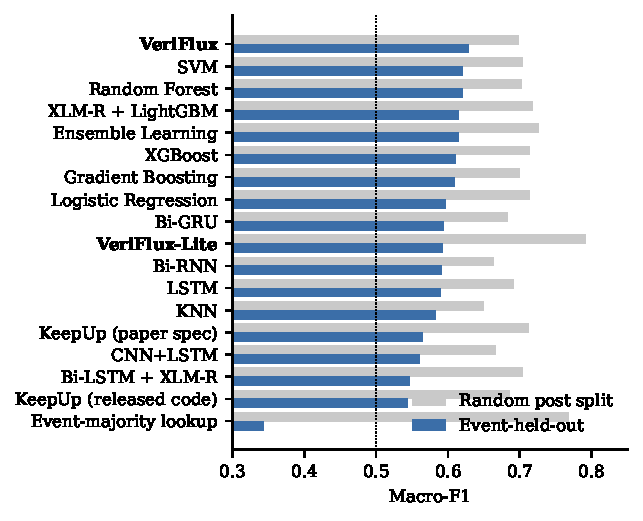
\includegraphics[width=\columnwidth]{figures/random_vs_event.pdf}
\caption{Macro-F1 under random and event-held-out splits for every model.}
\label{fig:gap}
\end{figure}

\subsection{Ablation}
Table~\ref{tab:ablation} isolates the components of both variants. In VeriFlux, removing the event contrast
lowers macro-F1 from 0.628 to 0.617 and AUC from 0.687 to 0.673, and makes the model much less stable across folds
(standard deviation 0.089 instead of 0.059). Removing the text embedding has the largest effect (0.572),
confirming that the frozen multilingual representation carries most of the cross-event signal. Removing the 38
named features does not reduce F1 (0.629), so in the kernel model their information is already present in the
embedding; they remain useful because they make the transformer-free variant possible and explainable.

In VeriFlux-Lite, both the contrast (0.579 without it) and the text prior (0.577 without it) help, and removing
both gives 0.568. User and engagement features matter most among the named families: dropping them costs 0.013
and 0.011 F1. Removing the evidence features does not hurt (0.595), which shows that claim-level evidence scores
do not transfer to new events, even though they are useful within known events. Replacing LightGBM with a random
forest improves the Lite model on unseen events (0.610), but we keep LightGBM because it supports the exact
TreeSHAP explanations used below.

\begin{table}[t]
\centering
\caption{VeriFlux ablation on the event-held-out protocol (15 folds)}
\label{tab:ablation}
\footnotesize
\begin{tabular}{lccc}
\toprule
Configuration & F1 & sd & AUC\\
\midrule
VeriFlux (full) & 0.628 & 0.059 & 0.687\\
VeriFlux w/o event contrast [E, F] & 0.617 & 0.089 & 0.673\\
VeriFlux w/o named features [E, Ec] & 0.629 & 0.056 & 0.690\\
VeriFlux w/o text embedding [F, Fc] & 0.572 & 0.053 & 0.626\\
VeriFlux-Lite (full) & 0.593 & 0.069 & 0.649\\
Lite classifier: Random Forest & 0.610 & 0.082 & 0.671\\
Lite only text prior & 0.581 & 0.060 & 0.614\\
Lite w/o contrast and text prior & 0.568 & 0.071 & 0.614\\
Lite w/o engagement features & 0.582 & 0.074 & 0.638\\
Lite w/o event contrast & 0.579 & 0.069 & 0.629\\
Lite w/o evidence features & 0.595 & 0.078 & 0.643\\
Lite w/o post\_claim features & 0.592 & 0.073 & 0.632\\
Lite w/o stance features & 0.590 & 0.079 & 0.649\\
Lite w/o text prior & 0.577 & 0.065 & 0.632\\
Lite w/o title features & 0.594 & 0.078 & 0.655\\
Lite w/o user features & 0.580 & 0.070 & 0.636\\
\bottomrule
\end{tabular}
\end{table}


\subsection{Comment budget (early-detection proxy)}
Because the comments in KeepUp have no timestamps, true time-based early detection cannot be evaluated. As a
proxy, we restricted VeriFlux-Lite to the first $k$ comments of each post in the order of the released sheet.
Fig.~\ref{fig:budget} shows that macro-F1 is essentially flat: 0.592 with no comments, 0.597 with 10 and 0.593 with
all of them. On unseen events the decision therefore rests on the post, its author and its engagement, which means
that the model can already be applied when a post is published, before readers have reacted. This proxy does not
reflect real arrival times and should be confirmed on timestamped data.

\begin{figure}[t]
\centering
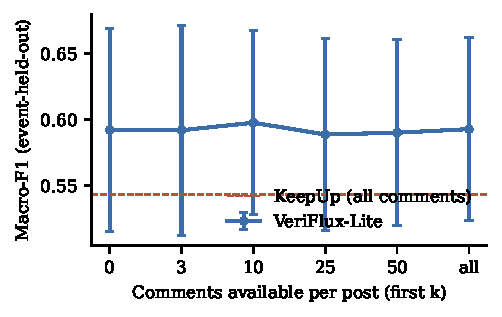
\includegraphics[width=\columnwidth]{figures/comment_budget.pdf}
\caption{Event-held-out macro-F1 of VeriFlux-Lite when only the first $k$ comments per post are available.}
\label{fig:budget}
\end{figure}

\subsection{Efficiency}
Table~\ref{tab:cost} reports the end-to-end CPU latency per post with batch size 1, with claim-level work
(retrieval and claim entailment) amortised over the average of 5.95 posts per event. KeepUp needs 6,028 ms per
post, dominated by running the stance network over every comment, and loads 4.4 GB of model weights. VeriFlux
needs 569 ms (\LatencyRatio{} times faster) with 2.0 GB of weights, and VeriFlux-Lite needs 204 ms (29.5 times
faster) with 0.9 GB. Both proposed models can therefore process thousands of posts per hour on an ordinary laptop.

\begin{table}[t]
\centering
\caption{CPU cost per post (Intel i7-8665U, batch size 1) and model size}
\label{tab:cost}
\footnotesize
\begin{tabular}{lcc}
\toprule
Component & ms/post & Weights MB\\
\midrule
KeepUp: claim-level (per claim) & 5545 & --\\
KeepUp: post-level & 5096 & --\\
KeepUp (total) & 6028 & 4356\\
VeriFlux-Lite / VeriFlux: claim-level (per claim) & 366 & --\\
VeriFlux-Lite / VeriFlux: post-level & 143 & --\\
VeriFlux-Lite (total) & 204 & 899\\
VeriFlux: XLM-R doc embedding + SVM & 364 & --\\
VeriFlux (total) & 569 & 2011\\
\bottomrule
\end{tabular}
\end{table}


\subsection{Explainability}
Fig.~\ref{fig:shap} and Table~\ref{tab:shap} show the global TreeSHAP importance of the VeriFlux-Lite features.
The text prior is the most influential feature, followed by the top-evidence NLI probabilities (contradiction,
neutral and entailment), the post--claim cosine similarity, the author's post count and the consistency term of
Eq.~(\ref{eq:consistency}). To test whether these explanations are faithful, we deleted the top-$k$ features of each
prediction and measured the change in predicted probability: removing the top 1, 3 and 5 features changes it by
0.118, 0.168 and 0.202, compared with 0.016, 0.037 and 0.052 for randomly chosen features. The feature rankings are
also stable, with a mean Spearman correlation of 0.78 (minimum 0.69) between folds. One tension is worth noting: the
evidence features rank highly because they separate posts within the training events, yet the ablation shows they
add nothing on new events. Explanations describe what the model uses, not necessarily what generalises.

\begin{figure}[t]
\centering
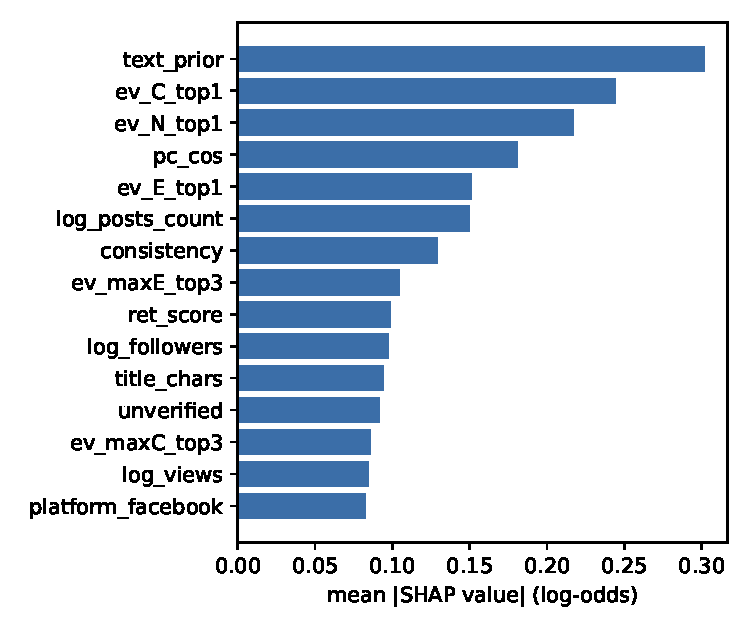
\includegraphics[width=\columnwidth]{figures/shap_global.pdf}
\caption{Global TreeSHAP importance of VeriFlux-Lite features on held-out events (seed-42 folds).}
\label{fig:shap}
\end{figure}
\begin{table}[t]
\centering
\caption{Ten most influential VeriFlux-Lite features (mean $|$SHAP$|$)}
\label{tab:shap}
\footnotesize
\begin{tabular}{lc}
\toprule
Feature & mean $|\phi|$\\
\midrule
text\_prior & 0.302\\
ev\_C\_top1 & 0.244\\
ev\_N\_top1 & 0.217\\
pc\_cos & 0.181\\
ev\_E\_top1 & 0.151\\
log\_posts\_count & 0.150\\
consistency & 0.129\\
ev\_maxE\_top3 & 0.104\\
ret\_score & 0.099\\
log\_followers & 0.098\\
\bottomrule
\end{tabular}
\end{table}


\subsection{Language-stratified results}
Table~\ref{tab:lang} breaks down event-held-out macro-F1 by title language. On the 664 English titles, VeriFlux
and random forest share the best score (0.629). The 332 Urdu-script titles are the hardest for every model
(0.48--0.54), and here the transformer-free VeriFlux-Lite is the best (0.539), probably because its character
n-gram text prior handles Urdu script better than the frozen XLM-R embedding. Roman Urdu has only 27 titles, so
its scores vary widely between models and no conclusion can be drawn from it.

\begin{table}[t]
\centering
\caption{Event-held-out macro-F1 by title language}
\label{tab:lang}
\footnotesize
\begin{tabular}{lccc}
\toprule
Model & English & Urdu & Roman Urdu\\
\midrule
KeepUp (released code) & 0.566 & 0.483 & 0.528\\
Random Forest & 0.629 & 0.479 & 0.673\\
SVM & 0.625 & 0.495 & 0.716\\
VeriFlux & 0.629 & 0.504 & 0.653\\
VeriFlux-Lite & 0.600 & 0.539 & 0.570\\
XGBoost & 0.609 & 0.530 & 0.724\\
\bottomrule
\end{tabular}
\end{table}


% ===========================================================================
\section{Discussion}
\label{sec:discussion}
The main finding of this study concerns evaluation rather than architecture. On KeepUp, a random split of posts
lets a model succeed by recognising which event a post belongs to: a lookup rule with no access to the post reaches
0.768 macro-F1, and every learned model drops sharply when events are held out. The 0.78 reported for KeepUp is
therefore not a measure of how well the framework would judge a new rumour, and our reproduction obtains
0.686--0.712 on random splits and 0.543--0.565 on unseen events. Part of the remaining gap to the published figure
is explained by the test-set epoch selection in the released code and by our frozen, rather than fine-tuned,
encoder.

When the protocol is fair, the large differences between architectures largely disappear. A heavy five-model
pipeline performs worse than an RBF-SVM on the same pooled embedding, and the best models are separated by less
than 0.01 macro-F1. VeriFlux is the best model on all event-held-out metrics, and its gain over KeepUp is
significant, but its gain over the SVM and random forest baselines is within statistical noise. Its practical
advantages are elsewhere: it is an order of magnitude cheaper than KeepUp, more stable across folds, and paired
with a transformer-free variant that is explained faithfully and works without comments. These properties match
the needs of fact-checking teams and newsrooms in low-resource settings, which have to triage many posts quickly
on ordinary hardware and need to justify each flag to an editor.

Compared with the reviewed literature, our results support the view that social signals are useful
\cite{almutair2025msdsi,nivedita2026hgcm}: in the ablation, user and engagement features are the most valuable
named families. They also qualify it. Claim-level evidence, the core of KeepUp and HCFND, did not transfer to new
events in our experiments, and the strong scores reported on random splits by most reviewed studies may overstate
real-world performance in the same way as on KeepUp. Only EvolveDetector \cite{ding2025evolvedetector} evaluates
on unseen events, and our work extends that evaluation to social context and to Urdu.

\section{Limitations and Future Work}
\label{sec:limits}
This study has several limitations. The dataset is small (1,024 posts and 172 events), so the confidence intervals
are wide and differences below about 0.03 macro-F1 cannot be resolved. The comments have no timestamps, so early
detection was approximated by a comment budget, and the engagement counters are final totals collected after the
fact. Because of the CPU-only environment, KeepUp and its stance network used frozen rather than fine-tuned
encoders, which may underestimate their best performance. The language tags are heuristic, the Roman-Urdu subset
is very small, and all results come from a single dataset. Finally, the final VeriFlux design was developed on
five of the reported folds.

Future work will address these points by re-collecting timestamped comments and engagement for true early
detection, fine-tuning multilingual stance and encoder models on a GPU, testing cross-dataset transfer to
FakeNewsNet and PHEME, running a human evaluation of the SHAP explanations with fact-checkers, and adding the images
and videos attached to many posts.

\section{Conclusion}
\label{sec:conclusion}
This paper studied social-context fake news detection on the multilingual KeepUp dataset. We re-implemented the
KeepUp framework and thirteen baselines under identical folds and showed that random post splits reward event
memorisation: a simple lookup rule nearly matches the published KeepUp score but fails on unseen events. We
proposed VeriFlux, which combines a frozen multilingual embedding with compact named features and an event-context
contrast. On unseen events VeriFlux achieved the best macro-F1 (\VFeventFone{}) and AUC (\VFeventAuc{}) of all
models, significantly above KeepUp (\KUeventFone{}) and on par with the strongest baselines, while running
\LatencyRatio{} times faster on a CPU. Its transformer-free variant VeriFlux-Lite achieved the best random-split
macro-F1 (\VFLrandomFone{}), works without comments and provides faithful TreeSHAP explanations. We hope that the
event-held-out protocol, the released code and the per-fold predictions will help future work report how well fake
news detectors generalise to the next event rather than the last one.

\section*{Code and Data Availability}
The source code, per-fold predictions and result tables are available in the authors' project repository. The
KeepUp dataset is available at
\url{https://github.com/sehrishsafdar/KeepUp-A-unified-framework-and-Dataset}.

\bibliographystyle{IEEEtran}
\bibliography{references}

\end{document}
